\section{Implementation}
\label{sec:streamimplementation}

\subsection{Abstractions choice}

As stated in the Architecture part, a stream processor is composed of one Iteratee in input and N Enumerators in output (one per child). Distribution is done using HTTP streaming on top of TCP. Custom processors on top of Iteratees have been selected over actors for several reasons.

First, actors does not handle back-pressure in a built-in way. But back-pressure is very important for our system in order to optimize resource consumption. Back-pressure is even
used from a parent's local journal to its children using the reactive MongoDB driver ReactiveMongo \footfullcite{bib:reactivemongo} that exposes methods returning Enumerators. It is really convenient to have only one composable abstraction to compose streams with back-pressure from MongoDB or from other processors.

Moreover, actors do not have a simple mechanism to sequentially compose asynchronous operations. When an actor processes a message and call an asynchronous function (which
returns a Future), it handle the next message in its mailbox meanwhile. An actor cannot "block in a non-blocking way" over asynchronous operations as Iteratees can. There exists
a solution using the Stash trait \footfullcite{bib:stashtrait} that allows to put in local memory the messages that we want to process after the current event has been asynchronously processed, but it is not fault-tolerant if the actor fails and not efficient as messages are swapped between the mailbox and the actor local memory (and not compatible with back-pressure).

In the end, Iteratees, Futures and Promises are better abstractions than actors to handle this problem.

\subsection{PathId serialization and deserialization into MongoDB}

The PathId Scala class is composed of the MongoDB id of the root event inserted in the Journal, plus a Vector of Int that represents the Path in the generational event tree.
A MongoDB id is an id created by the Scala MongoDB driver that is a 24-char hexadecimal string made with the current time plus a local incremental counter in order to guarantee that
each document id is unique and that the id of events are strictly ascendant to retain the order of insertion.

By default, MongoDB uses the \_id field of a document to store its unique id. Moreover, all MongoDB's collections have a default index on this field. Thus,
for simplicity and efficiency, we will serialize PathId to a hexadecimal string to put as a value of this \_id field. This serialization has to maintain the order
of events in a local journal. Indeed, ReactiveMongo's stream capabilities from MongoDB allows to get from MongoDB a stream of all the documents of a collection since a particular id in ascendant order according to ids. Therefore, this id has to be ascendant for all events of a local journal (to define the order, MongoDB does a simple String comparison from left to right).

The simplest way to do this is to first create the hexadecimal string as the root event 24-char id, and then append each integer of the path id as a padded 8-char byte. The padding allows easy deserialization.

With this serialization, events that have the same height in the tree have ids with the same number of chars (so in particular, all event ids generated by a processor have the same size). Moreover, locally in each local journal of processor, all events generated from a root event 01 created before root event 02 will have an id smaller than all events
generated from root event 02 (because they have the same size, and the root event id 01 has a higher id than 02 which are at the beginning of the hexadecimal string id). Furthermore,
sibling nodes in the event tree have an incremental number according to their creation order, so order is ensured in a substream. Figure \ref{fig:pathidserde} illustrates this serialization and ordering mechanism. With this model, for each input event, a processor can generate sub-events with an additional 4-byte part at the end of the PathId, so
for each event a processor can generate at maximum 2 power 32 events (around 4 billion events). This limit is considered to be sufficient for the use cases of the platform.

\begin{figure}[h]
  \begin{center} 
    \makebox[\textwidth]{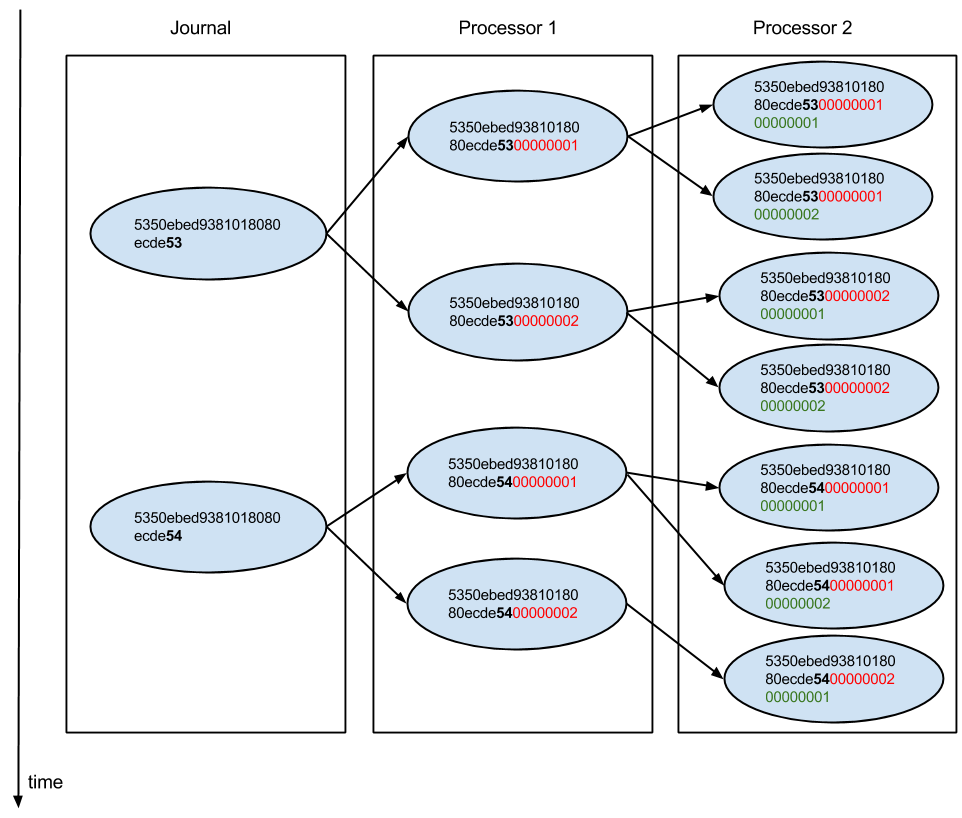
\includegraphics[width=1.0\textwidth]{img/pathidserde.png}}
    \caption{PathId serialization ensuring ordering in MongoDB local journals}
    \label{fig:pathidserde}
  \end{center}
\end{figure}

Listing \ref{lst:pathidserde} shows the code of Path Id and its serialization and deserialization.

\begin{listing}[h]
\begin{minted}[fontsize=\codesize, frame=lines, framesep=2mm]{scala}
case class PathId(rootEvent: String, path: Vector[Int])

object PathId {
  import reactivemongo.bson.utils.Converters
  import java.nio.ByteBuffer

  def apply(rootEvent: String): PathId = PathId(rootEvent, Vector.empty)

  def serialize(id: PathId): String = {
    val array = id.path
    val byteBuffer = ByteBuffer.allocate(array.length * 4)
    val intBuffer = byteBuffer.asIntBuffer
    intBuffer.put(array.toArray)
    byteBuffer.flip()

    id.rootEvent + Converters.hex2Str(byteBuffer.array())
  }

  def deserialize(str: String): PathId = {
    val (idStr, pathStr) = str.splitAt(12*2)

    val byteBuffer = ByteBuffer.allocate(4)
    val arrayBytes = Converters.str2Hex(pathStr)
    val path = arrayBytes.grouped(4).toVector map { bytes =>
      byteBuffer.put(bytes)
      byteBuffer.flip()
      val int = byteBuffer.getInt
      byteBuffer.clear()
      int
    }

    PathId(idStr, path)
  }

  val min = PathId("000000000000000000000000")
}
\end{minted}
\caption{PathId serialization and deserialization}
\label{lst:pathidserde}
\end{listing}


\subsection{Processors}

A stream processor is composed of one Iteratee in input and several Enumerators in output (one per child). 
In order to link the Iteratee with the Enumerators, we use the Promise abstraction to be able to fulfill manually a Future, and Scala STM \footfullcite{bib:scalastm} to handle concurrent accesses on shared state. 

When the Iteratee receives an input event, it processes it to create a substream that is flattened in-place into the main stream using the Enumeratee.mapFlatten helper. Moreover, the Enumeratee updatePathId is responsible of updating the PathId of each sub-event with the new level in the event tree.

Then, each sub-event goes through the effector method that is an Enumeratee executing asynchronously and sequentially the performAtomicSideEffect method (which is the insertion
in the local journal for persistent processors).

Last, sub-events go in the downstreamTrigger Iteratee that updates the state of each child according to the state transition diagram Figure \ref{fig:childstates}. Moreover, each
child that is UpToDate had previously registered a Promise to trigger in the consumersTrigger Map. This promise is linked to a Future that is returned by the Enumerator of a child
when this one is up to date. Thus, when we call promise.trySuccess(Some(outEvent)), the Future pushed in the Enumerator is fulfilled with the new sub-event (and so it will be sent
to the child).
\\

In the Enumerator corresponding to a child (the createOutStream method), when the code is called a new time (corresponding the ACK that previous events has been processed by the child in local mode,
or that the events are at least in the TCP send buffer in distributed mode), we check the state of the child. If it is UpToDate or WaitingForDownStreamAck, we register
a promise to be called when a new event will come in, and we put the Future linked to the promise into the Enumerator. This mechanism allows non-blocking long-polling.
If it is Late, we call the since method that retrieves the past events from the sinceId parameter. If the processor is a persistent stream processor,
it will directly take the past event streams from its MongoDB local journal and returns an Enumerator of it using the ReactiveMongo reactive driver. If the processor is
a side-effect stream processor, it will ask its parent for the past event streams, removing the last node of the path id and then filtering the substream via an offset in order to remove the already processed sub-events (as explained in the architecture part). 
Figure \ref{fig:createOutStream} illustrates this mechanism. 

\begin{figure}
  \begin{center} 
    \makebox[\textwidth]{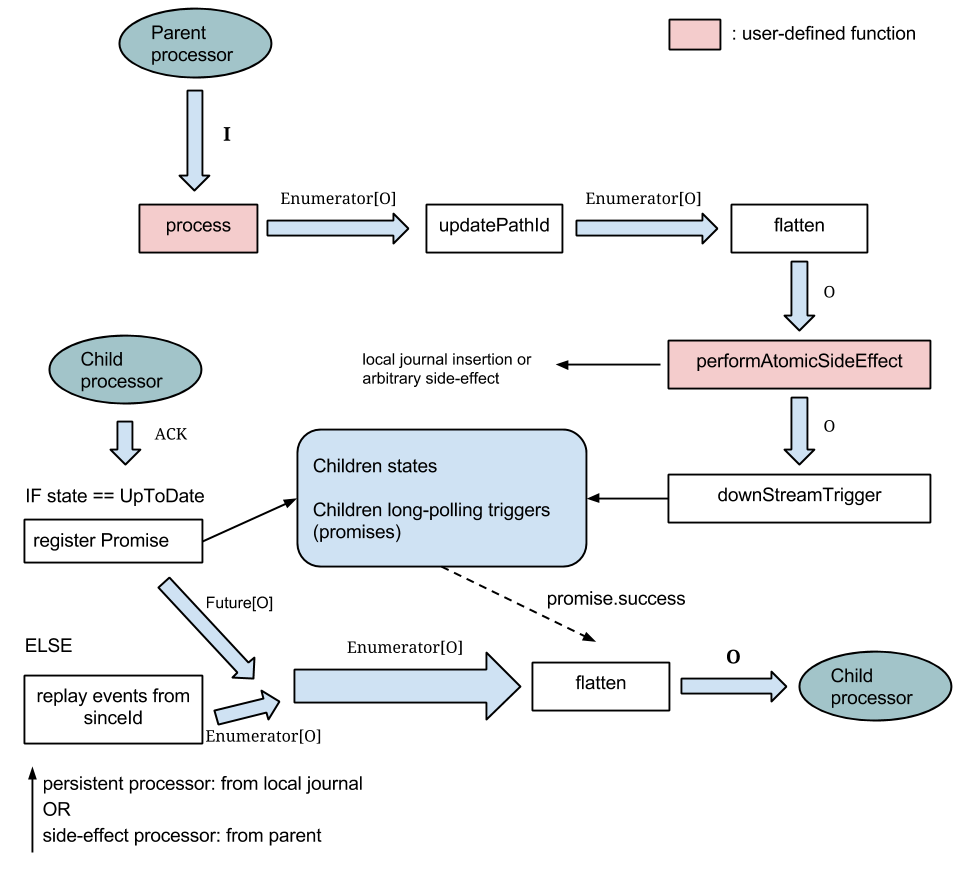
\includegraphics[width=1.0\textwidth]{img/createOutStream.png}}
    \caption{Processor implementation flow}
    \label{fig:createOutStream}
  \end{center}
\end{figure}

In order to share in a thread-safe way the Maps of Promises and States between the input Iteratee and the output Enumerators (so several concurrent threads), we use Scala STM (Software Transactional Memory) \footfullcite{bib:scalastm}. In a few words, a STM is an optimistic approach to concurrency that let all operations on a shared data structure to be done in parallel. An operation must be committed when it is finished. If there was another commit from another operation during this operation, the operation is aborted (rollback) and tried again. 
Using java.util.concurrent.ConcurrentHashMap is roughly equivalent for our use case.

Listing \ref{lst:processor} shows the code of the generic stream processor. Listing \ref{lst:psprocessor} shows the code of persistent stream processor and side-effect stream processor. 
\newpage

\begin{minted}[fontsize=\codesize, frame=lines, framesep=2mm]{scala}
// State for each consumer
sealed trait State
case object UpToDate extends State
case object WaitingForDownStreamAck extends State
case object Late extends State

trait Source[E] {
  def createOutStream(sinceId: PathId): Enumerator[E]
  def since(id: PathId, included: Boolean = false): Enumerator[E]
  def batchQuery(query: JsObject): Enumerator[E] = Enumerator.empty // TOOD: remove default
}

trait Evented[A] {
  def getId(a: A): PathId
  def updateId(a: A, id: PathId): A
  def serialize(a: A): JsObject
}

abstract class StreamProcessor[I, O](implicit ec: ExecutionContext, ei: Evented[I], eo: Evented[O])
   extends Source[O] {
  import scala.concurrent.stm._
  
  def since(id: PathId, included: Boolean = false): Enumerator[O]
  def process(event: I): Enumerator[O]
  def performAtomicSideEffect(event: O): Future[Unit]
  def getLastProcessedEventId(): Future[PathId]
  
  /*
   * Internals
   */

  val consumersTrigger = Ref(Map.empty[String, Promise[Option[O]]])
  val consumersState = Ref(Map.empty[String, State])

  def processor: Enumeratee[I, O] = {
    Enumeratee.mapFlatten[I](inEvent => process(inEvent) &> updatePathId)
  }

  def effector: Enumeratee[O, O] = {
    Enumeratee.mapM[O](outEvent => performAtomicSideEffect(outEvent) map (_ => outEvent))
  }

  def downstreamTrigger: Iteratee[O, Unit] =
    Iteratee.foreach[O] { outEvent =>
      consumersState.single transform { prev =>
        prev mapValues {
          case UpToDate => WaitingForDownStreamAck
          case WaitingForDownStreamAck => Late
          case Late => Late
        }
      }

      val promisesToTrigger = consumersTrigger.single.swap(Map.empty)
      promisesToTrigger foreach { case (_, promise) =>
        promise.trySuccess(Some(outEvent))
      }
    }

  def inStreamSink: Iteratee[I, Unit] = {
    processor ><> effector &>> downstreamTrigger
  }

  def createOutStream(sinceId: PathId): Enumerator[O] = {
    val consumerId = java.util.UUID.randomUUID().toString
    consumersState.single transform (prev => prev + (consumerId -> Late))

    StreamProcessorHelper.unfoldPathId(sinceId) { currentId =>
      val longPollingTrigger = promise[Option[O]]
      consumersTrigger.single.getAndTransform(prev => prev + (consumerId -> longPollingTrigger))

      consumersState.single.get.apply(consumerId) match {
        case WaitingForDownStreamAck | UpToDate =>
          // we are up to date with upstream, no need to pull from source
          consumersState.single.transform(prev => prev + (consumerId -> UpToDate))
          longPollingTrigger.future map { maybeEvent =>
            maybeEvent map (event => Some(currentId, Enumerator(event))) getOrElse 
              Some(currentId, Enumerator.empty[O])
          }

        case Late =>
          StreamProcessorHelper.headOption(since(currentId)) flatMap {
            case (None, _) =>
              // we don't have anything more to poll
              consumersState.single.transform(prev => prev + (consumerId -> UpToDate))
              longPollingTrigger.future map { maybeEvent =>
                maybeEvent map (event => Some(currentId, Enumerator(event))) getOrElse 
                  Some(currentId, Enumerator.empty[O])
              }

            case (Some(event), remainingEnum) =>
              // ignore promise
              consumersTrigger.single.getAndTransform(prev => prev - consumerId)
              // send next events
              Future.successful(Some(currentId, Enumerator(event) andThen remainingEnum))
          }
      }
    }
  }

  def updatePathId: Enumeratee[O, O] = StreamProcessorHelper.mapWithCounter { (outEvent, n) =>
    val oldId = eo.getId(outEvent)
    val newId = oldId.copy(path = oldId.path :+ n)
    eo.updateId(outEvent, newId)
  }
}
\end{minted}
\captionof{listing}{Processor implementation\label{lst:processor}}

\begin{minted}[fontsize=\codesize, frame=lines, framesep=2mm]{scala}
abstract class StreamProcessorWithReplayableSource[I, O]
  (implicit ec: ExecutionContext, ei: Evented[I], eo: Evented[O]) extends StreamProcessor[I, O] {

  val source: Source[I]

  def realtime(sinceId: PathId): Unit = {
    // restart the processor in case of failure
    def loopRestart(futIt: Future[Iteratee[I, Unit]]): Future[Iteratee[I, Unit]] = {
      futIt flatMap { _ =>
        getLastProcessedEventId() flatMap { lastId =>
          loopRestart(source.createOutStream(lastId) |>> inStreamSink)
        }
      }
    }

    loopRestart(source.createOutStream(sinceId) |>> inStreamSink)
  }

  def start(): Future[Unit] = {
    for {
      sinceId <- getLastProcessedEventId()
    } yield realtime(sinceId)
  }

}

abstract class SideEffectStreamProcessor[I, O](implicit ec: ExecutionContext,
    ei: Evented[I], eo: Evented[O]) extends StreamProcessorWithReplayableSource[I, O] {

  def since(id: PathId, included: Boolean = false): Enumerator[O] = {
    val ancestors = id.path.dropRight(1)

    val offset =
      if (id == PathId.min) 0
      else id.path.lastOption.getOrElse(0) + (if (included) 0 else 1)

    source.since(PathId(id.rootEvent, ancestors), included = true) &>
    processor &>
    Enumeratee.drop[O](offset)
  }
}

abstract class PersistentStreamProcessor[I, O](implicit ec: ExecutionContext, 
    ei: Evented[I], eo: Evented[O]) extends StreamProcessorWithReplayableSource[I, O] {

  def collection: JSONCollection
  def performAtomicSideEffect(event: O): Future[Unit] = 
    collection.insert(eo.serialize(event)) map (_ => ())
}
\end{minted}
\captionof{listing}{Persistent processor and side-effect processor implementation\label{lst:psprocessor}}


\subsection{Journal}

The Journal extends the StreamProcessor class but it differs from other processors by its way of handling input. Indeed, the Journal has multiple pushers (that pull from various data sources) which push events concurrently. To be sure to insert events with an increasing ordered id, we use Concurrent.broadcast that provides a channel to push events. Pushed events will go into an unique sequential pipeline that first creates a PathId for the event, and then inserts this event with its PathId to MongoDB (this is done by the journalSink Iteratee). Listing \ref{lst:journalimpl} shows the code of the Journal.

\begin{listing}[h]
\begin{minted}[fontsize=\codesize, frame=lines, framesep=2mm]{scala}
abstract class Journal[E](implicit ec: ExecutionContext, eo: Evented[E]) 
    extends StreamProcessor[E, E] {

  def collection: JSONCollection

  val (enum, channel) = Concurrent.broadcast[(E, Promise[E])]
  
  protected  def journalSink: Iteratee[(E, Promise[E]), Unit] = {
   Enumeratee.mapM[(E, Promise[E])] { case (event, p) =>
     // generate new event id to ensure that event are inserted in ascending order
     val bsonid = BSONObjectID.generate 
     val value = bsonid.value
     value(7) = Byte.MinValue // remove thread id to ensure sequentiality of events
     value(8) = Byte.MinValue
     val eventToInsert = eo.updateId(event, PathId(BSONObjectID(value).stringify))
     collection.insert(eo.serialize(eventToInsert)) map { _ =>
       p.trySuccess(eventToInsert)
       eventToInsert
     }
   } &>> downstreamTrigger
  }

  def start(): Future[Unit] = {
    enum |>> journalSink
    Future.successful()
  }


  def write(event: E): Future[E] = {
    val p = promise[E]
    channel.push(event, p)
    p.future
  }

  def writeSequentially(events: Seq[E]): Future[Option[E]] =
    Enumerator.enumerate(events) |>>> Iteratee.foldM(Option.empty[E]) { (_, event) =>
      write(event) map (Some(_))
    }

  def process(event: E): Enumerator[E] = Enumerator(event)
  override def inStreamSink = Iteratee.ignore // use journalSink instead
  def performAtomicSideEffect(event: E): Future[Unit] = Future.successful(())
  override def updatePathId = Enumeratee.map(identity) // 1 to 1 event generation relationship
}
\end{minted}
\caption{Journal implementation}
\label{lst:journalimpl}
\end{listing}


\subsection{Distribution}

Implementing point-to-point distribution is very easy thanks to Play Framework's helpers to transform an Enumerator into a HTTP Stream and a HTTP Stream into an Iteratee.

Basically, a parent processor can expose HTTP end-points for 2 functions: \verb|createOutStream| that push the infinite stream, and \verb|since| that allows child side-effect processors to ask for replay of past events.
\verb|createOutStream| can be mapped to an URL like \verb|/stream?pathId=<PATH_ID>| where PathId is the start point of the stream (non-included).
\verb|since| can be mapped to \verb|/since?pathId=<PATH_ID>&included=<BOOLEAN>| where PathId is the start point of the stream and included a boolean stating if we want the event
corresponding to PathId to be replayed. Contrary to \verb|createOutStream|, the since HTTP Stream is not infinite: it finishes when there is no more event to replay (no long-polling mechanism).
Listing \ref{lst:remoteparent} shows the implementation of such a HTTP interface.

\begin{listing}[h]
\begin{minted}[fontsize=\codesize, frame=lines, framesep=2mm]{scala}
object ProcessorHTTPInterface extends Controller {
  def stream(sinceId: String) = Action {
    val pathId = PathId.deserialize(sinceId)
    val enum = processor.createOutStream(pathId) &> Enumeratee.map(Json.toJson(_))
    Ok.chunked(enum)
  }

  def since(sinceId: String, included: Boolean) = Action {
    val pathId = PathId.deserialize(sinceId)
    val enum = processor.since(pathId, included) &> Enumeratee.map(Json.toJson(_))
    Ok.chunked(enum andThen Enumerator.eof)
  }
}
\end{minted}
\caption{Distributed processors: HTTP interface of a parent processor}
\label{lst:remoteparent}
\end{listing}

Concerning the child processor that has a remote parent, it must declare a remote source of type Source that can be transparently plugged into the StreamProcessor class. Listing \ref{lst:remotechild} shows the implementation of a remote source.

\begin{listing}[h]
\begin{minted}[fontsize=\codesize, frame=lines, framesep=2mm]{scala}
class RemoteParentProcessor extends Source[ZEvent] {
  val remoteParentUrl = "http://localhost:9001"

  def createOutStream(sinceId: PathId): Enumerator[ZEvent] = {
    val serializedId = PathId.serialize(sinceId)
    val url = s"$remoteParentUrl/stream?sinceId=$serializedId"
    getHttpStream(url)
  }

  def since(sinceId: PathId, included: Boolean = false) = {
    val serializedId = PathId.serialize(sinceId)
    val url = s"$remoteParentUrl/since?sinceId=$serializedId&included=$included"
    getHttpStream(url)
  }

  private def getHttpStream(url: String): Enumerator[ZEvent] = {
    val (it, enum) = Concurrent.joined[Array[Byte]]
    WS.url(url).get(_ => it).flatMap(_.run)
    enum &> Enumeratee.mapInput {
      case Input.El(chunk) =>
        val tryJs = Try(Json.parse(chunk))
        tryJs match {
          case Success(js) =>
            js.validate[ZEvent] map { ev =>
              Input.El(ev)
            } getOrElse {
              Input.Empty
            }

          case Failure(err) =>
            logger.error("Failure during json parsing", err)
            Input.Empty
        }

      case Input.Empty => Input.Empty
      case Input.EOF => Input.EOF
    }
  }
}
\end{minted}
\caption{Distributed processors: Remote source implementation of a child processor}
\label{lst:remotechild}
\end{listing}

Composability of Enumerators / Iteratees makes the distribution very easy (almost location transparent). Moreover, as explained in the architecture part, this code maintains
back-pressure with TCP-level ACK, which is very efficient.


\subsection{Example application}

The example application described in the architecture part has been implemented. The major part of the code is business specific and therefore will not be part of the report, but as an example Listing \ref{lst:exampleappimpl} shows the implementation of the FlatSnapshot side-effect processor.

\begin{listing}[h]
\begin{minted}[fontsize=\codesize, frame=lines, framesep=2mm]{scala}
object FlatSnapshot extends SideEffectStreamProcessor[ZEvent, ZEvent] with FlatSnapshotQuery {
  def collection = ReactiveMongoPlugin.db.collection[JSONCollection]("flat_snapshots")

  val logger: LazyLogger = LazyLogger.apply("api.FlatSnapshot")
  
  val source = Snapshot
  
  def getLastProcessedEventId(): Future[PathId] = {
    collection.find(Json.obj(), Json.obj(
      "_lastUpdateByEvent" -> 1)).sort(
      Json.obj("_lastUpdateByEvent" -> -1)).one[JsObject].map(_.flatMap { json =>
        (json \ "_lastUpdateByEvent").asOpt[PathId]
      }.getOrElse(PathId.min))
  }
  
  def process(event: ZEvent): Enumerator[ZEvent] = Enumerator(event)
  
  def performAtomicSideEffect(event: ZEvent): Future[Unit] = {
    val snapshot = ZSnapshot(event)
    if (!(event.body \ "archived").asOpt[Boolean].isEmpty) {
      FlatSnapshot.collection.remove(Json.obj("_id" -> snapshot.id)) map (_ => ())
    } else {
      FlatSnapshot.collection.save(ZSnapshot(event)) map (_ => ())
    }
  }

}
\end{minted}
\caption{Implementation of the FlatSnapshot side-effect processor}
\label{lst:exampleappimpl}
\end{listing}




